\documentclass[preprint,12pt]{elsarticle}

% --- packages (minimal, safe for elsarticle) ---
\usepackage{amsmath,amssymb}
\usepackage{graphicx}
\usepackage{booktabs}
\usepackage{array,tabularx,longtable,multirow,makecell,adjustbox}
\usepackage{float}
\usepackage{algorithm}
\usepackage{algpseudocode}
\usepackage{siunitx}
\usepackage{enumitem}
\usepackage{xcolor}
\usepackage{subcaption}
\usepackage{url}
\usepackage{xurl}
\usepackage{hyperref}

% --- hyperref / PDF-string fixes (author footnotes, subscripts, math) ---
\makeatletter
\pdfstringdefDisableCommands{%
  \def\corref#1{}% drop correspondence marks from PDF metadata
  \def\cnotenum#1{}%
  \def\@corref#1{}%
  \def\textsubscript#1{#1}% render F\textsubscript{1} as F1 in PDF metadata
}
\makeatother

\newcolumntype{C}{>{\centering\arraybackslash}X}


% --- column helpers ---
\newcolumntype{Y}{>{\raggedright\arraybackslash}X}

% --- manuscript-specific macros ---
\newcommand{\mtt}[1]{\texttt{#1}}
\newcommand{\NVDfeed}{\textsc{NVD} CVE API~2.0 / local CVSS cache}
\newcommand{\NVDfeeds}{\textsc{NVD} CVE API~2.0 / local CVSS caches}
\newcommand{\RepoLink}{\href{https://github.com/ErcanErkalkan/AI_Enabled__Standards_Aligned_Security_Risk_Management}{GitHub repository}}
\setlength{\emergencystretch}{2em}

\journal{Computer Standards \& Interfaces}

\begin{document}

\hypersetup{pageanchor=false}
\begin{frontmatter}

\title{A Machine-Readable Standards-Traceability Framework for Cybersecurity Risk Evidence in IoT Environments}

% authors & affiliations
\author[inst1]{Ercan Erkalkan\corref{cor1}}
\ead{ercan.erkalkan@marmara.edu.tr}
\cortext[cor1]{Corresponding author.}

\affiliation[inst1]{
organization={Marmara University, Vocational School of Technical Sciences, Department of Computer Technologies},
addressline={Mehmet Genc Kulliyesi},
city={Istanbul},
postcode={34865},
country={Turkey}
}

\begin{graphicalabstract}
\centering
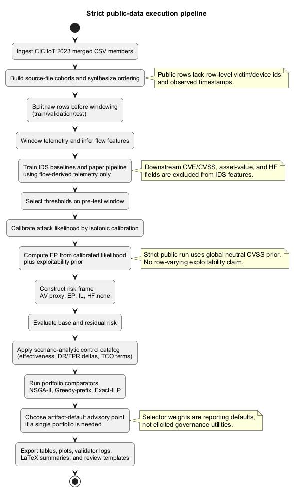
\includegraphics[width=0.92\textwidth,height=0.42\textheight,keepaspectratio]{figures/graphical_abstract.pdf}
\end{graphicalabstract}

\begin{abstract}
This study presents a machine-readable, standards-traceable framework for representing cybersecurity risk evidence. The proposed artifact encodes heterogeneous evidence into a UML/XMI knowledge model and structurally covers 93/93 ISO/IEC~27001:2022 Annex~A controls and 106/106 NIST CSF~2.0 subcategories through an executable Goal--Question--Metric mapping. To demonstrate operationalization under strict public-data constraints, the framework is instantiated on a telemetry-only CIC~IoT~2023 profile. This public experiment demonstrates representation-level traceability, executable validation, telemetry-derived evidence generation, and reporting/export reproducibility. It does not constitute a full empirical validation of the complete AV--EP--IL--HF risk formulation because the reported public profile uses a global neutral CVSS prior, telemetry-proxy asset values, no observed human-factor overlay, source-file cohort attribution, and synthesized ordering. The contribution therefore lies in the standards-traceable representation, structural validation, and reproducible reporting artifact rather than in deployment-level validation of all downstream risk factors.
\end{abstract}

\begin{highlights}
\item UML/XMI artifact captures standards-traceable cybersecurity risk evidence.
\item GQM mappings structurally cover 93 ISO and 106 NIST CSF 2.0 entries.
\item Executable validators check coverage, links, duplicates, and schema integrity.
\item Reporting exports preserve traceability from evidence to standards artifacts.
\item Portfolio layer exposes residual-risk and three-year TCO trade-offs.
\end{highlights}

\begin{keyword}
Cybersecurity risk representation \sep Standards traceability \sep ISO/IEC 27001 \sep
NIST CSF 2.0 \sep UML/XMI \sep Goal--Question--Metric \sep Interoperability
\end{keyword}

\end{frontmatter}
\clearpage
\hypersetup{pageanchor=true}

\section{Introduction}
\label{sec:introduction}

Cybersecurity risk management increasingly depends on heterogeneous evidence sources, including operational telemetry, vulnerability feeds, control metrics, audit records, and human-factor indicators. In practice, these evidence streams are generated by different tools, expressed at different levels of abstraction, and maintained in formats that are difficult to reconcile across governance, engineering, and audit workflows. Although widely used frameworks such as ISO/IEC~27001:2022, ISO/IEC~27005, and NIST CSF~2.0 provide structured guidance for risk-based decision making, they do not by themselves provide a machine-readable representation that links operational evidence to controls, risk constructs, and standards coverage in a reusable and verifiable form.

This gap becomes more pronounced in IoT-oriented environments, where asset heterogeneity, high event volume, and rapidly changing exposure conditions complicate the interpretation of security evidence. Intrusion detection systems, anomaly detectors, vulnerability intelligence, and awareness-related indicators can each provide useful signals, yet these signals are often consumed in isolation. As a result, organizations may achieve strong local analytics while still lacking a common representation that supports traceability, comparability, validation, and standards-aligned reporting. The problem is therefore not only one of detection quality, but also one of evidence integration, semantic consistency, and governance usability.

Existing risk registers and qualitative scoring schemes are often insufficient for this setting because they aggregate heterogeneous observations into coarse categories without preserving provenance, calibration, or explicit mappings to standards artifacts. At the same time, machine-learning outputs are frequently reported as standalone performance results rather than as components of a standards-traceable decision workflow. This creates a persistent disconnect between analytics, control selection, and audit-facing governance. A central need therefore remains for a structured artifact that can represent cybersecurity risk evidence in machine-readable form, validate its mappings to standards, and support downstream risk and portfolio analyses without losing traceability across the full evidence chain.

\subsection{Motivation and Problem Statement}
\label{sec:intro-motivation}
\label{sec:intro-problem}

The main difficulty in contemporary cybersecurity risk management is not only the availability of security signals, but the lack of a common, machine-readable structure for representing them in a standards-aligned manner. In IoT-oriented environments, telemetry summaries, vulnerability descriptors, audit observations, control metrics, and human-factor indicators are typically produced by separate tools and maintained with different semantics. Although ISO/IEC~27001:2022, ISO/IEC~27005, and the NIST RMF encourage traceable and repeatable risk assessment, they do not by themselves define an interoperable representation layer that can transform heterogeneous operational evidence into reusable risk artifacts with explicit links to controls, governance objectives, and standards coverage.

This limitation affects not only technical analysis but also validation and governance. Risk registers and qualitative scoring schemes often compress heterogeneous observations into coarse categories, which weakens provenance, comparability, and calibration across assets and time. At the same time, AI-enabled security analytics can generate anomaly scores, class probabilities, and related evidence streams, yet these outputs are frequently consumed as isolated analytical products rather than as elements of a standards-traceable evidence chain. Without a unifying representation and validation mechanism, such signals remain difficult to reconcile with formal control mappings, difficult to reuse across audit and reporting workflows, and difficult to explain consistently in governance settings.

Three practical gaps follow from this situation. First, operational evidence, vulnerability context, and socio-technical indicators are rarely represented within a single auditable structure that preserves semantics and provenance. Second, mappings from evidence items to ISO/IEC~27001 and NIST CSF objectives are often incomplete or non-machine-readable, which limits validation, interoperability, and reporting reuse. Third, downstream quantitative risk and portfolio analyses are commonly performed without an explicit representation layer that maintains end-to-end traceability from raw evidence to control recommendations. The method proposed in response to these gaps is referred to throughout the manuscript as the proposed standards-traceable risk framework.

\subsection{Research Questions}
\label{sec:research-questions}

To address the identified representation, validation, and governance gaps, the study is structured around four research questions:

\begin{enumerate}[label=\textbf{RQ\arabic*},ref=RQ\arabic*,labelsep=0.4em,leftmargin=2.6em]
  \item \label{RQ1} \textbf{Representation:} How can heterogeneous cybersecurity evidence---including assets, threats, vulnerabilities, events, controls, and metric classes---be encoded in a reusable, machine-readable, and standards-aligned knowledge model?
  \item \label{RQ2} \textbf{Validation and standards traceability:} How can mappings from evidence items to ISO/IEC~27001:2022 and NIST CSF~2.0 artifacts be represented and validated so that coverage, integrity, and traceability can be demonstrated in a reproducible manner?
  \item \label{RQ3} \textbf{Telemetry-evidence transformation:} How can telemetry-derived security evidence be transformed into traceable risk-facing quantities and budget-aware scenario comparisons while preserving provenance and making inactive or proxy risk factors explicit?
  \item \label{RQ4} \textbf{Governance-facing export provisioning:} How can decision rationales, validation outputs, and standards-linked metrics be exported in traceable reporting-facing forms that could support downstream audit, dashboard, reporting, or continuous-improvement workflows?
\end{enumerate}

For \ref{RQ2}, evaluation focuses on standards-coverage and validation evidence, including mapping completeness, broken-link checks, duplicate-row checks, dangling-row checks, machine-readable consistency across UML/XMI and GQM artifacts, and bidirectional ISO--NIST informative-reference consistency. These checks establish representation-level integrity and cross-framework consistency; they do not by themselves prove that every evidence-to-control mapping is the only possible interpretation. For \ref{RQ3}, evaluation focuses on telemetry-only evidence-generation quality and downstream scenario-analysis behaviour, including residual risk, three-year TCO, detection rate (DR), false-positive rate (FPR), $F_{1}$ score, area under the receiver-operating characteristic curve (AUROC), precision--recall AUC (PR-AUC), and the Brier score. Operating thresholds are selected on the pre-test window and then evaluated on the hold-out test split. For \ref{RQ4}, evaluation focuses on whether the generated tables, plots, validator outputs, and schema-linked exports preserve links from controls and subcategories to metrics, residual-risk summaries, and portfolio quantities in reporting-facing form. This checks export-layer traceability and packaging; it does not by itself establish auditor uptake, end-user usability, or deployed tool integration.

\subsection{Scope and Contributions}
\label{sec:intro-gap}

The empirical scope of the study is intentionally framed as a public-data operationalization and representation-level evaluation of the proposed artifact rather than as a full deployment validation of the complete risk engine. The framework is instantiated on IoT-heavy network telemetry with offline vulnerability enrichment using the public CIC~IoT~2023 corpus, which provides multi-scenario flow records for benign and malicious traffic in heterogeneous IoT deployments~\cite{Neto2023_CICIoT2023,CICIoT2023_Web}. In the reported artifact run, all 63 merged CSV members are consumed under a resource-aware row budget. The headline evaluation is telemetry-only and boundary-safe: intrusion-detection models use only flow-derived telemetry, while CVE/CVSS, human-factor, and asset-value terms are introduced only after classification in the downstream representation and risk layers. The public release also provides an attack-victim inventory, which is retained as provenance metadata, but the released CSV files do not expose row-level victim identifiers and therefore cannot be deterministically joined back to individual flows. Accordingly, the strict public-data profile treats the 63 merged members as source-file cohorts, derives telemetry-proxy asset values, disables event-only CVE surrogates, and falls back to a global neutral CVSS prior unless a curated asset- or timestamp-level manifest is supplied. The strict public evaluation should therefore be interpreted as a representation-level and telemetry-evidence demonstration. It checks structural coverage, traceability, executable consistency, and reproducible exports, but it does not empirically validate row-varying CVSS exploitability, verified enterprise asset values, observed human-factor effects, or measured control intervention effects. External validity beyond IoT-oriented environments is discussed qualitatively rather than claimed empirically.

Within this scope, the study makes four main contributions:

\begin{enumerate}[label=\textbf{C\arabic*.},ref=C\arabic*,leftmargin=*]
  \item \label{contrib1} \textbf{Machine-readable standards-traceability artifact:} A reusable UML/XMI-based representation for cybersecurity risk evidence that encodes assets, threats, vulnerabilities, events, controls, and metric classes in a standards-aligned knowledge model linked to ISO/IEC~27005 and NIST RMF concepts.
  
  \item \label{contrib2} \textbf{Validation and mapping layer:} We provide an executable structural validation layer that checks standards coverage, identifier consistency, evidence-to-metric linkage, and report-generation completeness. A machine-readable Goal--Question--Metric mapping and validation workflow provides structural coverage for \textbf{all ISO/IEC~27001:2022 Annex~A controls (93)} and \textbf{all NIST CSF~2.0 subcategories (106)}. This contribution concerns reproducible standards traceability and structural consistency rather than a compliance oracle.

  \item \label{contrib3} \textbf{Telemetry-evidence-to-risk demonstration with explicit activation boundaries:} An auditable transformation architecture is provided for hosting AV, EP, IL, and optional HF terms within a standards-linked risk representation. In the strict public-data profile, only the telemetry-derived likelihood path is empirically activated. CVSS exploitability is represented by a constant global neutral prior, asset value is represented by a telemetry-derived source-cohort proxy, and the human-factor term is inactive because no observed HF overlay is available. Therefore, this contribution should be interpreted as a representation-level and telemetry-evidence demonstration, not as a full public-data validation of all AV--EP--IL--HF factors.

  \item \label{contrib4} \textbf{Budget-constrained portfolio comparison as a scenario-analytic operational demonstration:} A downstream advisory layer that compares control portfolios under a portfolio-level Gordon--Loeb bound using configurable control-catalog assumptions. On the reported strict public-data profile, NSGA-II returns a 61-point trade-off set (HV=31{,}436.9), Greedy returns a 14-point prefix frontier (HV=30{,}810.2), and Exact-ILP returns a 16-point log-space frontier (HV=28{,}970.3) on the $(\text{ResidualRisk},\ \mathrm{TCO}^{\mathrm{ctrl}}_{3y})$ plane. Any single recommended point is treated as an artifact-default advisory selection rather than as a governance-optimal prescription; under the default selector, the chosen NSGA-II point yields 4.5\% lower mean residual risk and 5.0\% higher three-year control TCO relative to the matched-budget Greedy comparator.
\end{enumerate}

\subsection{Background and Related Work}
\label{sec:related}

The most relevant literature for the present study spans four intersecting streams: standards-oriented risk frameworks, quantitative risk transformation methods, AI-generated security evidence, and traceability-oriented metric and portfolio workflows. Rather than treating these streams as isolated topics, the present review emphasizes how they relate to a central Computer Standards \& Interfaces concern: whether heterogeneous cybersecurity evidence can be represented, validated, and reused in a machine-readable, standards-aligned form. The discussion therefore focuses not only on analytical capability, but also on representation structure, validation logic, interoperability potential, and governance-facing reuse.

%--------------------------------------------------
\subsubsection{Standards-Oriented Risk Frameworks and Representation Gaps}
\label{sec:risk-foundations}

Enterprise risk management standards such as ISO~31000 and its predecessor AS/NZS~4360 define generic processes for establishing context, identifying risks, analyzing likelihood and impact, and selecting treatments across organizational domains~\cite{ISO31000,ASNZS4360}. ISO/IEC~27005 specializes these concepts for information security by introducing asset inventories, threat and vulnerability catalogs, likelihood--impact structures, and iterative treatment cycles coupled to ISO/IEC~27001 controls~\cite{ISO27005}. NIST SP~800-30 and related guidance similarly emphasize cyclical assessment, response, and monitoring, with explicit links to control baselines~\cite{NIST80030}. Frameworks such as OCTAVE FORTE operationalize self-directed profiling and workshop-driven analysis aligned with risk management tasks~\cite{OCTAVEFORTE}.

\noindent\textbf{Gap:} Standards-oriented frameworks define processes, concepts, and control contexts, but they stop short of providing a reusable machine-readable representation layer that can encode heterogeneous operational evidence, validate mappings, and support interoperable downstream reuse across audit, governance, and analytical workflows.

%--------------------------------------------------
\subsubsection{Quantitative Risk Transformation and Machine-Readable Gaps}
\label{sec:quant-fair}

Quantitative risk analysis methods extend qualitative schemes by expressing risk as a function of probability and impact. Classical approaches, including Annualized Loss Expectancy, decision-theoretic formulations, and analytic hierarchy process (AHP)-based weighting, assign monetary valuations to assets and estimate loss frequencies to support investment decisions~\cite{Courtney1985NBS}. The Gordon--Loeb model demonstrates that optimal security expenditure rarely exceeds approximately $37\,\%$ of the expected loss for a given information asset, providing a widely cited economic bound on security investment~\cite{Gordon2002_SecInvest}. Later work introduces Bayesian and Monte Carlo formulations that propagate uncertainty in frequency and magnitude parameters and define scenario-based loss distributions for cyber risk~\cite{Radanliev2020}.

The Factor Analysis of Information Risk (FAIR) methodology structures loss events into explicit frequency and magnitude factors, supported by a taxonomy and process guidance for calibrating parameters in currency terms~\cite{FAIR}. In practice, FAIR-style models are often combined with high-level frameworks such as ISO/IEC~27001 or the NIST Cybersecurity Framework to improve risk quantification, but typically with organization-specific adaptations and without a standard machine-readable representation~\cite{ParenteEtAl2025_JISA_FRAPE,KhalilEtAl2025_JISA_CyberROAD}.

\noindent\textbf{Gap:} Quantitative and FAIR-like approaches provide economic structure and risk-factor decomposition, but they rarely specify how heterogeneous evidence should be represented in machine-readable form before numerical transformation, how such transformations remain traceable to standards artifacts, or how validation and interoperability should be preserved across the representation-to-risk pipeline.

%--------------------------------------------------
\subsubsection{AI-Generated Security Evidence and Analytical Transformation}
\label{sec:ai-ids}

Machine learning and, more recently, deep learning have significantly advanced intrusion detection and anomaly detection. Early expert-system and hybrid anomaly--misuse detectors demonstrated that combining statistical models with signature-based rules yields improved coverage compared with purely rule-based systems~\cite{Depren2005ESWA_IDS}. Subsequent surveys synthesize supervised, unsupervised, and hybrid intrusion-detection approaches, emphasizing the importance of feature engineering, traffic representation, and dataset realism~\cite{Tsai2009_ESWA_Review}. Recent work reports that machine-learning-based intrusion detection can improve detection performance but also highlights the need for explainability, controllability, and robust evaluation against adversarial behavior~\cite{Apruzzese2022}.

For time-series and industrial contexts, interpretable and calibrated anomaly detectors have received particular attention. Extensive evaluations of unsupervised time-series anomaly detection methods underline the importance of calibrated probability outputs and reliability analysis~\cite{Mejri2024_ESWA_TSANOM}. Interpretable deep-learning architectures for industrial control and SCADA environments attach explanation mechanisms or structured feature attributions to sequence models in order to meet audit and safety requirements~\cite{Wadinger2024_ESWA_AID}. Lightweight designs for intrusion detection tailored to Internet of Things deployments illustrate how resource constraints and deployment topologies affect model architecture and performance trade-offs~\cite{Li2024_ESWA_LightIDS}. Incremental and online learning approaches further address non-stationary traffic patterns and concept drift in streaming settings~\cite{Wang2011ESWA_IncSVM}.

\noindent\textbf{Gap:} AI-enhanced intrusion-detection research primarily improves analytical performance, calibration, and interpretability, yet the resulting signals are still often treated as endpoint outputs rather than as machine-readable evidence objects that can be validated, linked to standards artifacts, and reused consistently in downstream risk and governance workflows.

%--------------------------------------------------
\subsubsection{Traceability, GQM, and Budget-Constrained Downstream Decision Support}
\label{sec:cost-gqm}

Cost-benefit analysis and optimization for security controls build on economic risk models and metrics-based governance. The Gordon--Loeb framework provides a theoretical upper bound on rational security investment relative to expected loss~\cite{Gordon2002_SecInvest}. Multi-objective optimization techniques, such as the Non-Dominated Sorting Genetic Algorithm~II (NSGA-II), have been applied to security-hardening and configuration problems to balance conflicting objectives like risk reduction, financial cost, and usability~\cite{Rabiei2023_ESWA_NSGAII}. These formulations often encode control-selection decisions as binary vectors and evaluate fitness based on simulated attack graphs or scenario analyses, producing Pareto fronts rather than single-point recommendations.

The Goal--Question--Metric (GQM) paradigm provides a complementary perspective by deriving measurable indicators from high-level goals through intermediate questions~\cite{Basili2014GQM}. Security-focused adaptations of GQM define key performance indicators for policy compliance, incident response, and awareness programs and encourage alignment between organizational objectives and technical metrics. However, many applications remain at the level of conceptual scorecards or dashboards and do not embed metrics into a formal data model or an explicit optimization loop that selects control portfolios.

\noindent\textbf{Gap:} Existing GQM and cost-effectiveness studies provide valuable metric hierarchies and portfolio heuristics, but they seldom define a full standards-traceable workflow in which evidence items, mappings, validation checks, and downstream portfolio comparisons remain connected through a common machine-readable artifact.

%--------------------------------------------------
\subsubsection{Summary of Gaps and Positioning}
\label{sec:summary-gaps}

Across these four streams, a common limitation persists: cybersecurity risk workflows are often rich in concepts, metrics, or analytics, but comparatively weak in machine-readable representation, validation logic, and interoperable reuse. Standards-oriented frameworks define governance structure without fully specifying reusable evidence artifacts; quantitative approaches transform risk factors without fully preserving representation-level traceability; AI-based studies generate strong analytical signals without consistently turning them into standards-linked evidence objects; and GQM or portfolio studies support metrics and decisions without maintaining an explicit end-to-end representation chain.

The present study is positioned at this intersection. The central contribution is not merely a quantitative risk score or an optimization routine, but a machine-readable standards-traceability framework that connects heterogeneous cybersecurity evidence to controls, governance objectives, and downstream decision processes. In this positioning, the UML/XMI knowledge model provides the representation layer, the GQM matrix and validator provide the validation layer, the AV$\times$EP$\times$IL formulation provides the traceable transformation layer, and the Gordon--Loeb-bounded portfolio analysis serves as a downstream operational demonstration rather than as the sole core contribution. This combination distinguishes the framework from prior studies that address only one or two of these layers in isolation.


The remainder of the manuscript details the architecture and methodology (Section~\ref{sec:methods}), presents empirical results (Section~\ref{sec:results}), discusses implications, limitations, and future work (Section~\ref{sec:discussion}), and closes with concluding remarks (Section~\ref{sec:conclusions}).


% ==================== Methods (condensed core) ====================
\section{Methods}
\label{sec:methods}

This section describes the proposed framework as a standards-traceable representation, validation, and downstream operationalization architecture. The presentation is organized around four cooperating layers: a machine-readable knowledge model, a standards-mapping and validation layer, a traceable quantitative risk-transformation layer, and a downstream advisory layer used for portfolio comparison under explicit budget constraints. Figure~\ref{fig:four_layer} summarizes this organization, while detailed algorithmic settings and extended experimental protocols are provided in the Appendices and in the public repository (\RepoLink).

\begin{figure}[H]
  \centering
  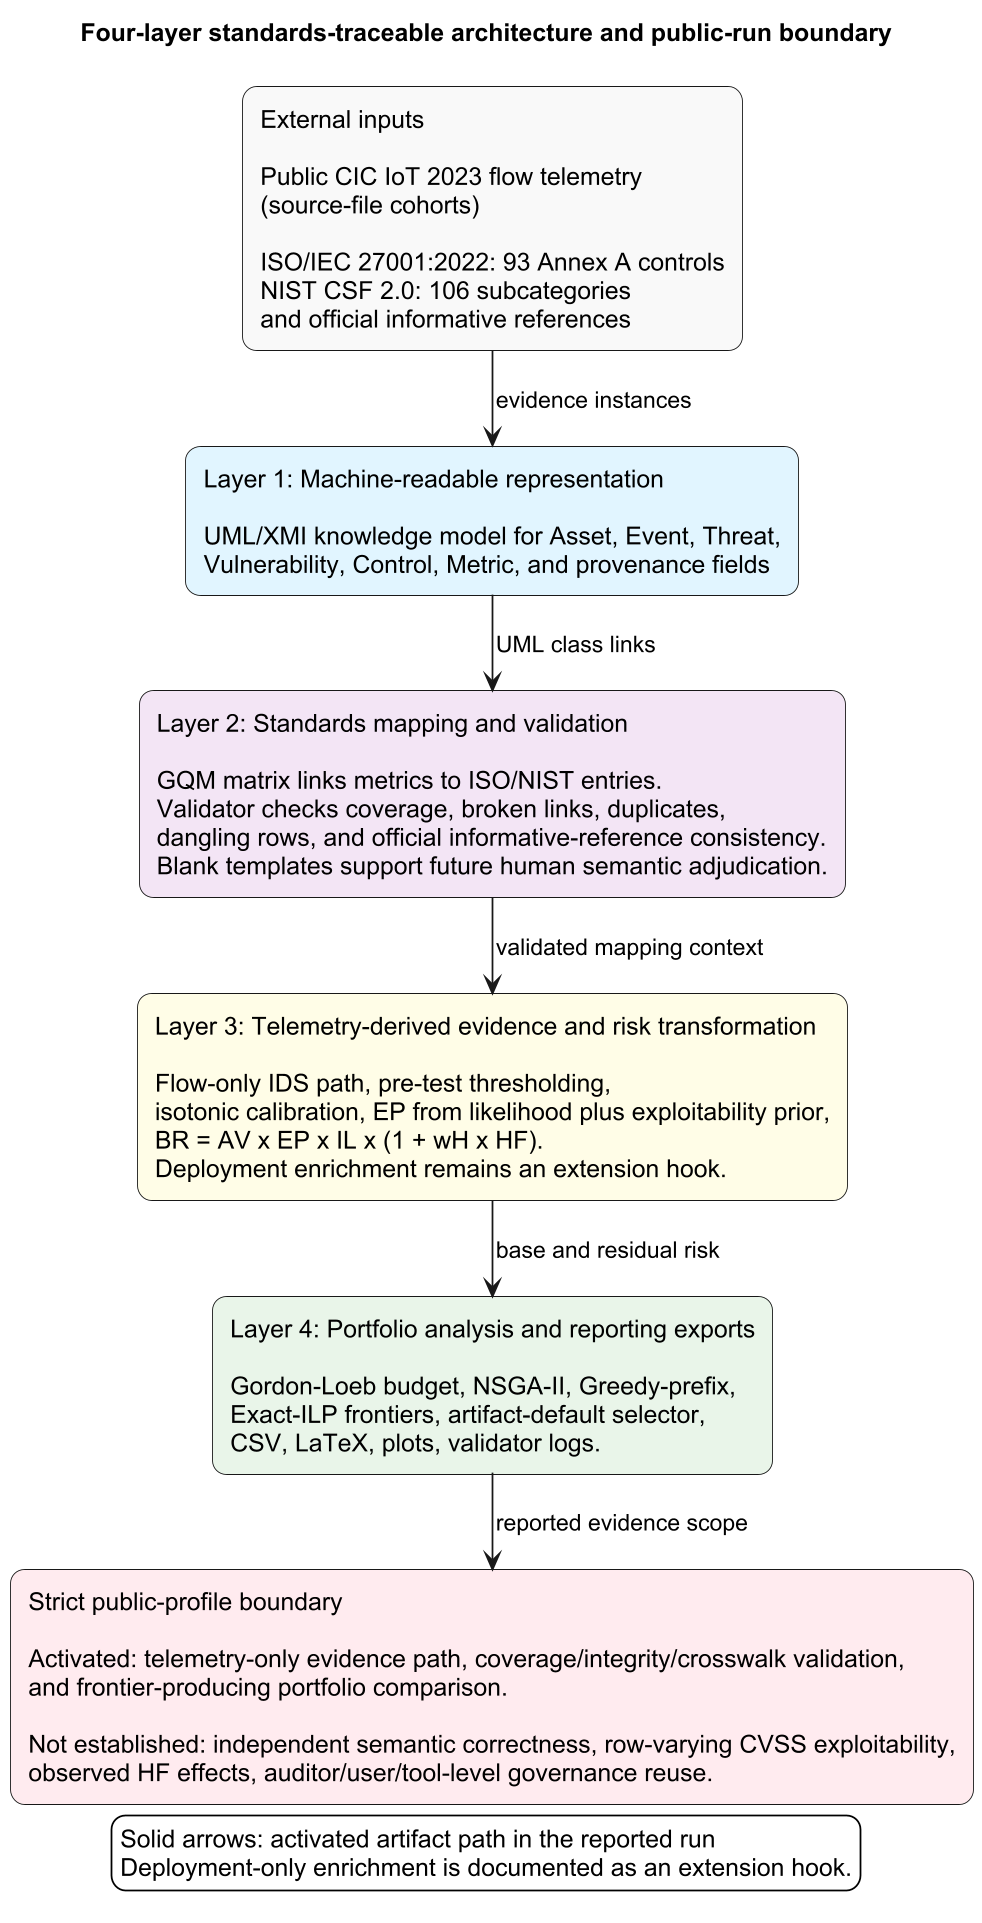
\includegraphics[width=\linewidth,height=0.82\textheight,keepaspectratio]{figures/figure_1_standards_traceability_architecture.png}
  \caption{Four-layer standards-traceable architecture and strict public-profile evidence boundary. The figure distinguishes the activated artifact path from deployment-only enrichment hooks and unestablished validation claims.}
  \label{fig:four_layer}
\end{figure}


% --------------------------------------------------
\subsection{Overall Architecture}
\label{sec:overall}

The proposed framework is organized as a four-layer standards-traceable architecture that addresses the representation, validation, transformation, and downstream-use questions posed in RQ1--RQ4 (Fig.~\ref{fig:four_layer}). The framework is intentionally structured so that analytical modules remain subordinate to the representation and traceability logic rather than defining the full contribution by themselves.

\begin{enumerate}[label=\arabic*),leftmargin=*]
  \item \textbf{Machine-Readable Knowledge Representation Layer} (blue) encodes ISO/IEC~27005 and NIST RMF entities such as \textit{Asset}, \textit{Threat}, \textit{Vulnerability}, \textit{Event}, \textit{Risk}, and \textit{RiskTreatment}, together with associated metric classes. This layer provides the common representation artifact through which heterogeneous cybersecurity evidence can be expressed in a reusable and standards-aligned form.

  \item \textbf{Standards-Mapping and Validation Layer} (purple) links evidence items and metric classes to ISO/IEC~27001:2022 Annex~A controls and NIST CSF~2.0 subcategories through a machine-readable Goal--Question--Metric structure. This layer supports coverage validation, integrity checks, and traceability demonstration across standards artifacts and implementation objects.

  \item \textbf{Traceable Quantitative Risk-Transformation Layer} (orange) converts represented evidence into auditable quantitative risk constructs using Asset Value (AV), Event Probability (EP), Impact Level (IL), and optional Human-Factor (HF) terms, together with residual-risk and cost formulations. This layer serves as the transformation bridge between represented evidence and governance-relevant decision variables.

  \item \textbf{Downstream Portfolio-Advisory Layer} (green) consumes the transformed risk quantities and compares feasible control portfolios under a Gordon--Loeb-type spending bound. In this architecture, portfolio optimization is treated as a downstream operational use of the represented and validated evidence chain rather than as the sole defining contribution of the framework.
\end{enumerate}

Connectors in Fig.~\ref{fig:four_layer} denote the activated artifact path and the retained traceability links across these layers. This organization ensures that detections, mappings, risk transformations, and portfolio outputs can be reconstructed from shared evidence objects and standards-linked artifacts during audit, governance, and reporting workflows.
% --------------------------------------------------
\subsection{Standards-Aligned Data Model (UML)}
\label{sec:uml}
The UML-based data model serves as the machine-readable representation core of the framework and consists of a \emph{conceptual layer} and a \emph{metric layer}, as illustrated in Figs.~\ref{fig:conceptual_uml} and~\ref{fig:metric_uml}.

\begin{itemize}[leftmargin=*]
  \item \texttt{Asset}, \texttt{Threat}, \texttt{Vulnerability}, \texttt{Event}, \texttt{Impact}, and \texttt{Risk};
  \item \texttt{RiskTreatment}, \texttt{SecurityRequirement}, and \texttt{SecurityObjective}, together with provenance attributes and relationships.
\end{itemize}

Cardinalities follow IEEE~1016-2017 conventions; for example, a \texttt{Threat} may target one or more \texttt{Vulnerability} instances, while a \texttt{RiskTreatment} may mitigate several \texttt{Risk} instances. These associations align the model with ISO/IEC~27005 Tasks~2--5 (context, assessment, treatment, and monitoring) and NIST RMF steps.

The metric layer introduces five core metric classes and one human-factor class:

\begin{itemize}[leftmargin=*]
  \item \texttt{AssetValue}, \texttt{EventPotential}, and \texttt{ImpactLevel} hold the quantitative factors used to compute base risk;
  \item \texttt{RiskReductionLevel} and \texttt{CostMetrics} capture residual risk and economic consequences after the application of controls;
  \item \texttt{HumanFactorMetric} aggregates socio-technical indicators such as phishing outcomes, policy violations, and awareness-training completion.
\end{itemize}

Each association in the metric layer is annotated with a verb (\emph{evaluates}, \emph{assesses}, \emph{quantifies}, or \emph{captures}) and is linked to a Goal--Question--Metric (GQM) entry, enabling machine-readable traceability between standards, metrics, and controls. A complete XMI export of the UML schema is provided in the public repository.

\begin{figure}[H]
  \centering
  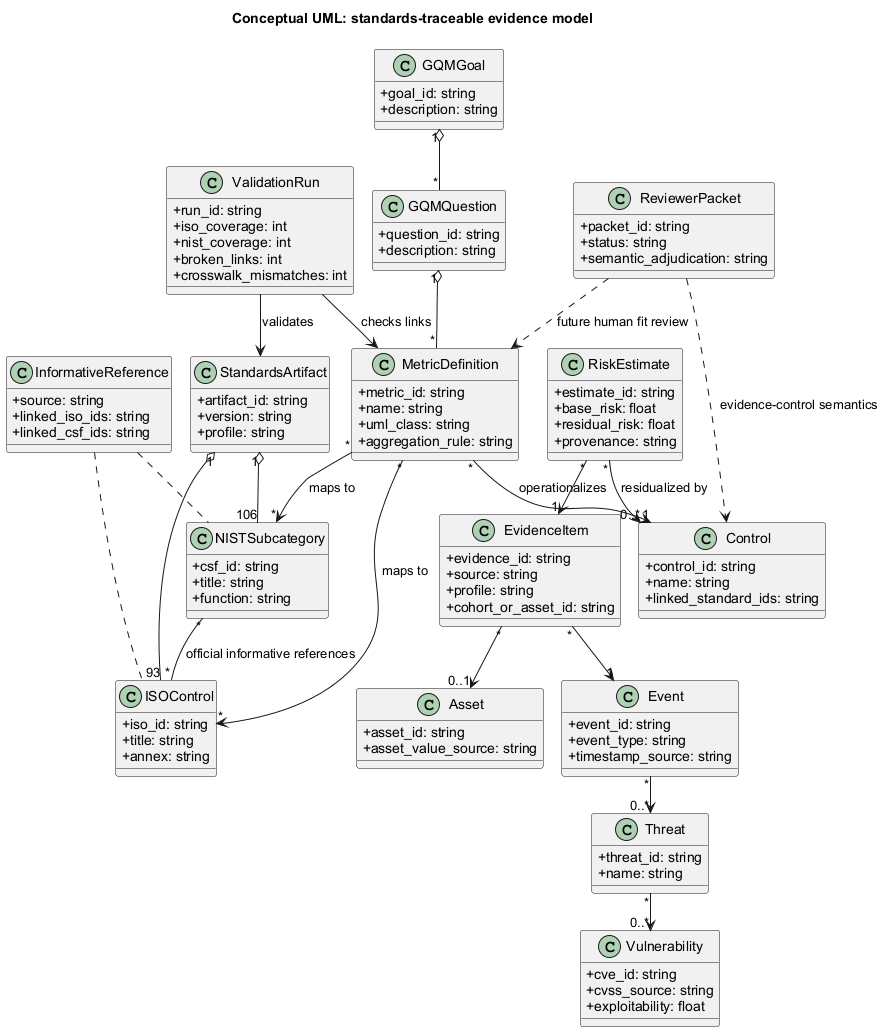
\includegraphics[width=\linewidth,height=0.78\textheight,keepaspectratio]{figures/figure_2a_conceptual_uml.png}
  \caption{Conceptual UML layer for the standards-traceable evidence model. It links standards artifacts, GQM questions and metrics, evidence items, risk estimates, controls, and structural validation runs.}
  \label{fig:conceptual_uml}
\end{figure}

\begin{figure}[H]
  \centering
  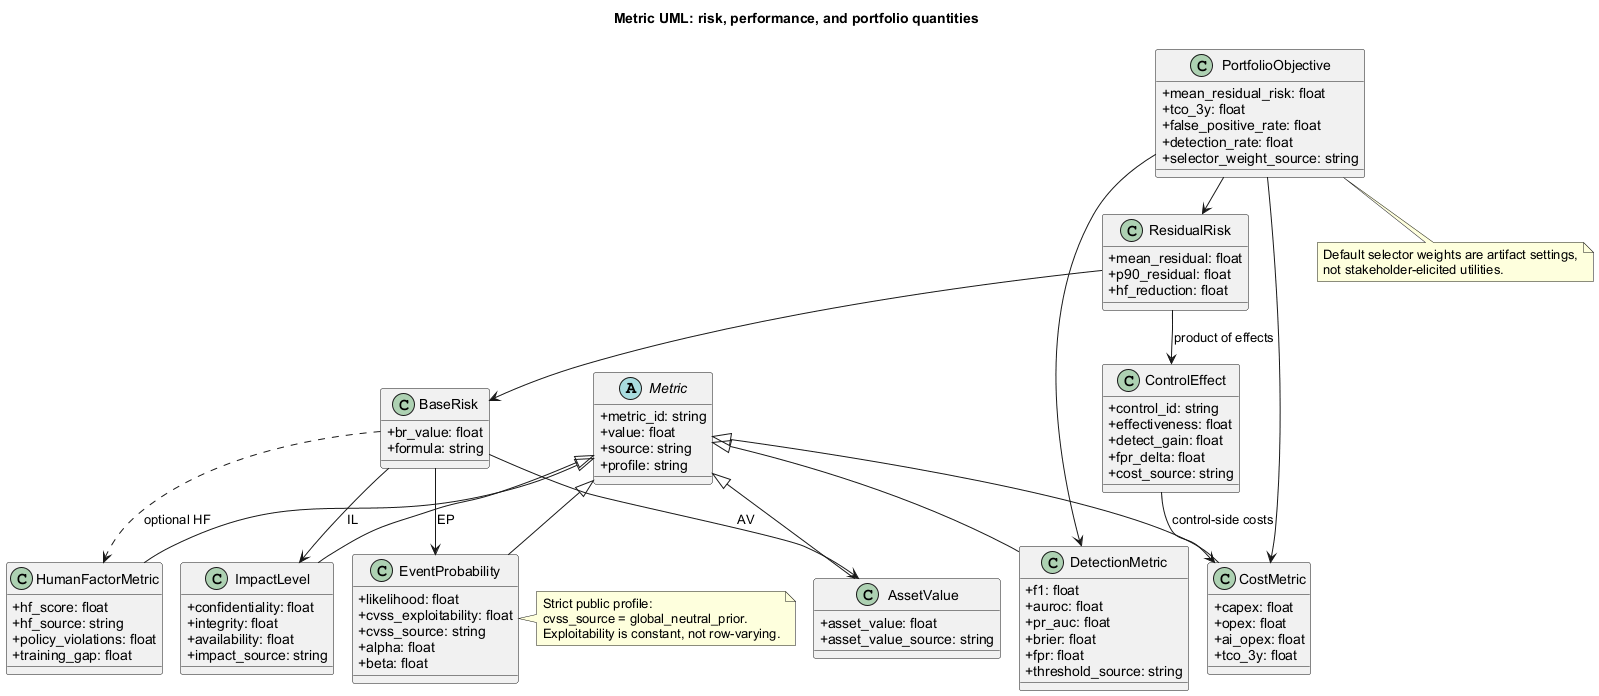
\includegraphics[width=\linewidth,height=0.72\textheight,keepaspectratio]{figures/figure_2b_metric_uml.png}
  \caption{Metric UML layer for risk, performance, and portfolio quantities. Source fields distinguish telemetry-derived values, neutral public-data priors, optional human-factor overlays, scenario-analytic control effects, and artifact-default selector weights.}
  \label{fig:metric_uml}
\end{figure}


% --------------------------------------------------
\subsection{Traceable Risk Transformation and Downstream Portfolio Comparison}
\label{sec:math_human}

\begin{table*}[t]
\centering
\caption{Risk-factor activation status in the strict public-data profile.}
\label{tab:risk_factor_activation}
\small
\setlength{\tabcolsep}{3pt}
\begin{tabularx}{\textwidth}{@{}p{0.13\textwidth}XXX@{}}
\toprule
Risk factor & Public-profile implementation & Empirical status & Permitted claim \\
\midrule
AV & Telemetry-derived source-cohort proxy & Proxy only; no verified enterprise asset register & Representation and proxy demonstration \\
EP telemetry likelihood & IDS/anomaly score from flow-derived features & Empirically activated & Telemetry-derived likelihood path demonstrated \\
EP exploitability / CVSS & Global neutral prior & Constant; no row-varying CVE/CVSS linkage & Extension hook represented, not validated \\
IL & Catalog/scenario-based impact scaling & Scenario assumption & Scenario-analysis demonstration only \\
HF & \texttt{HF:none} & Inactive; no observed HF overlay & HF slot represented, not empirically validated \\
Device identity & Source-file cohort & Surrogate; no row-level device attribution & Cohort-level provenance only \\
Time & Synthesized ordering & Surrogate; no true wall-clock chronology & Ordered hold-out demonstration only \\
Control effectiveness & Configurable catalog coefficients & Planning assumption; not measured intervention effect & Portfolio scenario exploration only \\
\bottomrule
\end{tabularx}
\end{table*}

This layer performs the traceable transformation from represented cybersecurity evidence to governance-relevant quantitative risk variables. The formulation combines asset value, event probability, technical impact, and optional human-factor terms in a manner that remains compatible with ISO/IEC~27001, ISO/IEC~27005, and NIST CSF~2.0, while preserving the distinction between telemetry-derived evidence and downstream enrichment variables used for risk and portfolio analysis. In deployment settings, these enrichment terms can be populated from asset registers, curated CVE/CVSS manifests, and observed human-factor overlays. In the strict public-data profile reported here, however, the non-telemetry terms are only partially activated: asset value is instantiated through a tagged telemetry proxy, CVSS-based exploitability falls back to a neutral prior, and the human-factor overlay remains inactive. Table~\ref{tab:risk_factor_activation} defines which risk factors are empirically activated in the strict public-data profile and which factors are represented only as provenance-preserving extension hooks. Accordingly, the reported experiment should not be read as a full validation of the complete AV--EP--IL--HF risk formulation. The public run therefore validates the telemetry-derived evidence path and representation logic rather than a full empirical activation of all downstream factors.

\paragraph{Asset value.}
Each asset $i$ has a raw monetary valuation $\tilde v_i \ge 0$ obtained either from an asset register or, in public-data profiles without business valuations, from a tagged proxy source. A normalized asset-value factor
\begin{equation}
  \mathrm{AV}_i =
    \frac{\tilde v_i - \min(\tilde v)}
         {\max(\tilde v) - \min(\tilde v)}
  \label{eq:av}
\end{equation}
is used in the risk score, where the denominator spans the valuation range of the considered assets.

\paragraph{Event probability.}
For each event type $j$ (e.g., an attack family or exploitation scenario), event probability is expressed as
\begin{equation}
  \mathrm{EP}_j =
    \sigma\!\bigl(\alpha\,\mathrm{likelihood}_j + \beta\,\mathrm{exploitability}_j\bigr),
  \qquad
  \sigma(x) = \frac{1}{1+\mathrm{e}^{-x}},
  \label{eq:ep}
\end{equation}
where $\mathrm{likelihood}_j$ is derived from telemetry and historical frequency indicators, and $\mathrm{exploitability}_j$ is derived from CVSS-based vulnerability attributes (e.g., attack vector and complexity). In enriched deployment profiles where exploitability varies across observations, coefficients $\alpha$ and $\beta$ can be fitted by logistic regression on labeled historical events. In the strict public-data profile reported here, however, all rows carry the same \texttt{global\_neutral\_prior} CVSS tag, so $\mathrm{exploitability}_j$ is constant across the evaluation set. The reported public run should therefore be read as a telemetry-driven calibration of the likelihood term within the EP architecture, not as a full empirical validation of a row-varying multi-factor exploitability component.

\paragraph{Impact level with human factors.}
For each scenario $k$ associated with an event, confidentiality, integrity, and availability impacts are represented as normalized scores $e_{Ck}, e_{Ik}, e_{Ak} \in [0,1]$ derived from CVSS impact metrics. A human-factor term $\mathrm{HF}_k \in [0,1]$ summarizes socio-technical indicators such as phishing-simulation failure ratios, policy-violation densities, and training/culture indices; higher values indicate higher residual socio-technical risk. The combined impact level is
\begin{equation}
  \mathrm{IL}_k =
      w_C e_{Ck} + w_I e_{Ik} + w_A e_{Ak} + w_H \mathrm{HF}_k,
  \qquad
  w_C + w_I + w_A + w_H = 1,
  \label{eq:il}
\end{equation}
where $(w_C,w_I,w_A,w_H)$ are governance-defined weights. The public repository documents the optional human-factor overlay columns used when deployment-specific HF data are available.

\paragraph{Base risk and expected loss.}
Within the transformation layer, the represented evidence factors are combined into auditable base-risk and expected-loss quantities. The base risk associated with asset $i$, event $j$, and scenario $k$ is defined as
\begin{equation}
  \mathrm{BR}_{ijk} =
      \mathrm{AV}_i \cdot \mathrm{EP}_j \cdot \mathrm{IL}_k.
  \label{eq:br}
\end{equation}
In monetary terms, the corresponding expected loss is
\begin{equation}
  \mathbb{E}[\mathrm{Loss}_{ijk}] = \tilde v_i \cdot \mathrm{EP}_j \cdot \mathrm{IL}_k.
  \label{eq:eloss}
\end{equation}
Portfolio-level expected loss over a planning window $W$ (e.g., one quarter) aggregates Eq.~\eqref{eq:eloss} across assets, events, and scenarios using exposure multipliers and scenario weights; the full expression is given in Appendix~\ref{app:calibration}.

\paragraph{Residual risk and cost.}
For a given control portfolio $K$, the transformation layer also produces downstream decision variables describing residual risk and control-side cost. Each control $m \in K$ has an effectiveness coefficient $\eta_m \in [0,1]$ that reflects the fraction of risk addressed by that control under the modeled conditions. A human-factor reduction coefficient $\eta_H \in [0,1]$ captures the effect of awareness and culture interventions. In the shared artifact, these control effectiveness and cost terms are configurable scenario-analytic defaults stored in \texttt{control\_catalog.csv}; they should be interpreted as transparent planning assumptions rather than as intervention effects estimated from the public CIC~IoT~2023 release.
\begin{equation}
  \mathrm{ResidualRisk}(K) =
      \mathrm{BR}_{ijk}\,(1-\eta_H)
      \prod_{m \in K}\!\bigl(1-\eta_m\bigr).
  \label{eq:resrisk}
\end{equation}
The associated risk-reduction level is
\begin{equation}
  \mathrm{RRL}(K) =
      \frac{\mathrm{BR}_{ijk} - \mathrm{ResidualRisk}(K)}
           {\mathrm{BR}_{ijk}}.
  \label{eq:rrl}
\end{equation}

The three-year control-side Total Cost of Ownership of portfolio $K$ is decomposed into capital and recurring operating expenditures:
\begin{equation}
  \mathrm{TCO}^{\mathrm{ctrl}}_{3y}(K) =
      \mathrm{CapEx}_K + 3\,\mathrm{OpEx}_K + 3\,\mathrm{OpEx}^{\mathrm{AI}}_K,
  \label{eq:cm}
\end{equation}
where $\mathrm{OpEx}^{\mathrm{AI}}_K$ includes compute, storage, and staffing costs required by the AI components. Hidden-loss terms are not estimated from the public CIC~IoT~2023 release and are therefore kept outside the strict reported TCO metric.

\paragraph{Downstream portfolio-comparison constraint and objectives.}
At the downstream decision-support stage, security investment is constrained by a Gordon--Loeb bound~\cite{Gordon2002_SecInvest}:
\begin{equation}
  \sum_{m \in K} \mathrm{CapEx}_m \;\le\; \gamma\ \mathbb{E}[\mathrm{Loss}]_{W},
  \qquad \gamma \approx 0.37,
  \label{eq:gl_portfolio}
\end{equation}
where $\mathbb{E}[\mathrm{Loss}]_{W}$ denotes the aggregated expected loss over window $W$. Optional asset-level and rolling-window variants are defined in Appendix~\ref{app:calibration}.

For downstream portfolio comparison, the framework evaluates each feasible portfolio through a four-objective vector:
\begin{equation}
  \mathbf{f}(K) = \bigl(f_1, f_2, f_3, f_4\bigr)
                = \bigl(\mathrm{ResidualRisk}(K),\ \mathrm{TCO}^{\mathrm{ctrl}}_{3y}(K),\ \mathrm{FPR},\ -\mathrm{DR}\bigr),
  \label{eq:objectives_mo}
\end{equation}
where DR (detection rate) and FPR (false-positive rate) are portfolio-level scenario metrics initialized from the underlying intrusion-detection models and adjusted by control-catalog deltas. In the present architecture, NSGA-II~\cite{Deb2002_NSGAII} is used as a downstream portfolio-comparison mechanism rather than as the primary representation artifact itself. Using a binary decision vector $\mathbf{x}\in\{0,1\}^{M}$, where $x_m=1$ selects control $m$, the procedure approximates a feasible trade-off frontier under the constraint~\eqref{eq:gl_portfolio}. A concise pseudo-code listing is retained in Algorithm~\ref{alg:nsgaii}; full hyperparameter grids and sensitivity analyses are moved to Appendix~\ref{app:opt-details}.

\begin{algorithm}[H]
\caption{NSGA--II as a downstream portfolio-comparison procedure under the Gordon--Loeb bound}
\label{alg:nsgaii}
\begin{algorithmic}[1]
\Require Initial population size $P$, number of generations $G$, control universe $\{1,\dots,M\}$, Gordon--Loeb budget $B$.
\State Initialize population $\mathcal{P}_0$ of binary portfolios satisfying Eq.~\eqref{eq:gl_portfolio}.
\For{$t=0$ to $G-1$}
  \State Evaluate objectives $\mathbf{f}(K)$ for all $K\in\mathcal{P}_t$ via Eqs.~\eqref{eq:resrisk}--\eqref{eq:objectives_mo}.
  \State Apply non-dominated sorting and crowding-distance assignment.
  \State Select parents by binary tournament on (rank, crowding distance).
  \State Apply crossover and mutation to generate offspring; repair GL-violating portfolios to satisfy Eq.~\eqref{eq:gl_portfolio}.
  \State Form $\mathcal{P}_{t+1}$ by merging parents and offspring and keeping the best $P$ individuals.
\EndFor
\State \Return Approximate Pareto front from the final population.
\end{algorithmic}
\end{algorithm}


% --------------------------------------------------
\subsection{Datasets and Preprocessing}
\label{sec:dataset}

The framework is instantiated on heterogeneous IoT telemetry enriched with vulnerability information. Two primary data sources are used: the CIC~IoT~2023 dataset for network flows and the NVD vulnerability feed for CVE attributes.

\paragraph{CIC~IoT~2023.}
CIC~IoT~2023~\cite{Neto2023_CICIoT2023,CICIoT2023_Web} is a large-scale benchmark for intrusion detection in IoT environments. The corpus includes traffic from 105 IoT devices, covering benign activity and 33 attack scenarios grouped into seven categories (DDoS, DoS, reconnaissance, web, brute-force, spoofing, and Mirai variants). Each bidirectional flow is represented by statistical and protocol features such as duration, packet and byte counts, packet rates, TCP flag counts, and application/transport protocol indicators.

In the present study, flows are labeled as benign or malicious according to the original scenario annotations. The reported resource-aware evaluation ingests all 63 members of the merged CSV release with a uniform 1{,}000-row cap per member, yielding 63{,}000 raw rows across 63 source files and 33 event types. Because the public CSV release does not expose victim-device identifiers, the strict artifact run treats each merged member as a \emph{source-file cohort} rather than a verified physical device. Missing timestamps are synthesized when absent; numeric flow statistics are retained in their original numeric form; telemetry-only windows are constructed for IDS training; and missing numeric values are imputed. Asset values are not read from an enterprise register in this public profile; instead, a telemetry-derived asset-value proxy is derived from per-cohort traffic statistics and tagged as \texttt{asset\_value\_source=telemetry\_proxy}. The official victims inventory is preserved as side-car metadata, but it cannot be joined to the public CSV rows because those rows do not encode victim-device identifiers. Raw rows are first partitioned into training, validation, and test segments; because the public profile uses source-file cohorts as surrogate assets, split boundaries are aligned to cohort changes before window construction so that neither raw flows nor windowed samples straddle partitions. Windowing then produces 61{,}488 samples using 25-flow windows per cohort, with 44 source-file cohorts in training, 10 in validation, and 9 in test. This design preserves boundary safety for telemetry-derived evidence generation, but it does not by itself supply verified asset-level business values, device-level CVE joins, or observed organizational human-factor measurements.

\paragraph{NVD vulnerability feed.}
The NVD CVE API~2.0 and locally provisioned CVSS records~\cite{NVD_CVE_API_2025} provide CVE identifiers, textual descriptions, CVSS~v3.1 base metrics, and affected configurations. The implemented artifact accepts event-level, asset-level, or asset+timestamp-level CVE maps. However, event-level joins are label-derived on the public CIC~IoT~2023 release and therefore leak attack identity if used in headline evaluation. The strict reported profile disables such event-only surrogates and only admits curated asset- or timestamp-level joins; when those are unavailable, all rows fall back to a global neutral CVSS prior tagged as \texttt{cvss\_source=global\_neutral\_prior}. In the reported strict public profile, this fallback applies to every row, so $\mathrm{exploitability}_j$ is constant across the evaluation set. The public run therefore preserves the exploitability field for provenance and downstream compatibility, but it does not empirically identify a row-varying CVSS effect in Eq.~\eqref{eq:ep}. These attributes feed into the event-probability and impact-level components in Eqs.~\eqref{eq:ep} and~\eqref{eq:il}. Vulnerability records are linked to the UML entities \texttt{Vulnerability}, \texttt{Event}, and \texttt{ImpactLevel}. Device-level attribution remains possible only when a curator can provide a compatible per-asset manifest external to the public CSV release.

\paragraph{Preprocessing pipeline.}
Figure~\ref{fig:ai_pipeline} sketches the end-to-end ingestion and decision pipeline. Raw CIC~IoT~2023 flow files are first ingested, then transformed into UML-aligned instances with provenance tags. The implemented artifact normalizes column names, synthesizes timestamps when needed, records provenance for cohort identifiers, asset values, CVSS sources, and human-factor overlays, imputes missing numeric values, partitions raw rows before any window construction, and then builds rolling windows using mean/std/last-value telemetry summaries. Crucially, the telemetry-only configuration excludes asset-value, CVSS, and human-factor columns from the IDS feature matrix; these fields are preserved only in the metadata consumed by the downstream risk layer. In the strict public-data profile, that metadata records non-telemetry terms as proxies, neutral priors, or inactive overlays rather than as empirically observed factors. Where required by specific models, telemetry features are additionally standardized within the training partition. The same split logic is reused for all models and baselines to ensure comparability.

\begin{figure}[H]
  \centering
  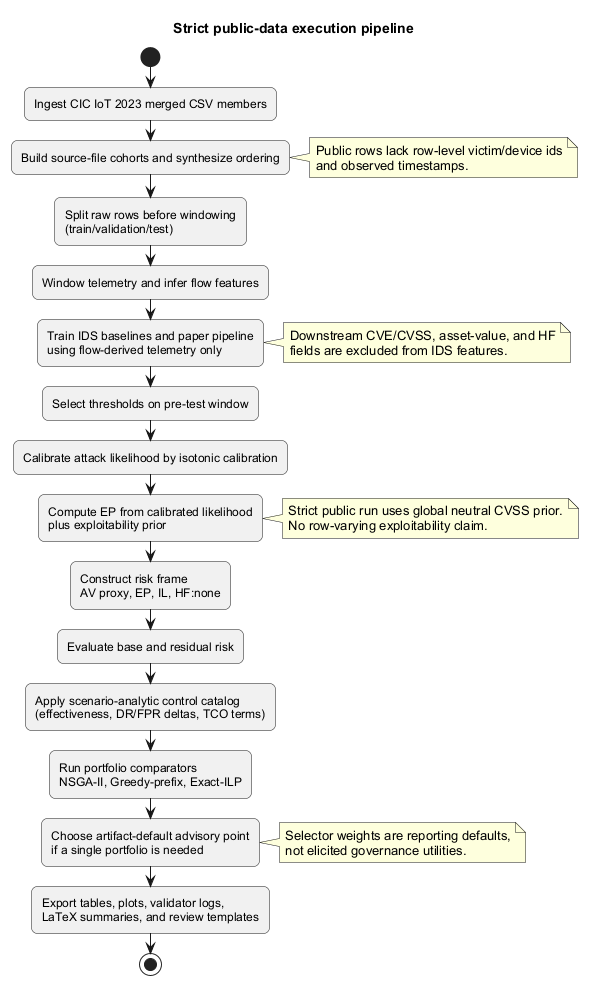
\includegraphics[width=\linewidth,height=0.78\textheight,keepaspectratio]{figures/figure_3_telemetry_to_reporting_pipeline.png}
  \caption{Strict public-data execution pipeline from raw IoT telemetry through leakage-safe IDS training, calibrated likelihood estimation, source-tagged risk construction, scenario-analytic portfolio comparison, and reporting exports.}
  \label{fig:ai_pipeline}
\end{figure}


% --------------------------------------------------
\subsection{Machine-Learning Pipeline}
\label{sec:model-details}

\subsubsection{Classifier-Agnostic Telemetry Evidence Interface}
The framework does not require a specific IDS architecture. A telemetry scorer is treated as an evidence generator if it provides: (i) an asset or source-cohort identifier, (ii) a timestamp or surrogate ordering index, (iii) a calibrated maliciousness or anomaly score, (iv) a thresholded alert label when needed, and (v) provenance metadata linking the score to the input feature window and model configuration.

\subsubsection{Artifact-Default Telemetry Scorer}
The AI layer combines an unsupervised neural anomaly detector with a supervised gradient-boosted risk scorer. The aim is to convert raw flow telemetry into calibrated attack-likelihood estimates and then combine those estimates with separately curated risk metadata in a standards-aligned risk layer that supports downstream portfolio comparison. The resulting pipeline is presented as one telemetry-only operationalization of the artifact, not as a claim that it is the strongest standalone classifier among all tested baselines.

\paragraph{LSTM-based anomaly detection.}
Temporal patterns of benign traffic are modeled with a Long Short-Term Memory (LSTM) network~\cite{Hochreiter1997_LSTM}. Input sequences consist of fixed-length windows of numeric flow features per asset (25-flow windows in the reported resource-aware profile). The implemented detector is a two-layer LSTM regressor followed by a small feed-forward head; it is trained only on benign windows to predict the final feature vector in each sequence using mean-squared error and the Adam optimizer~\cite{Kingma2014_Adam}. The per-window anomaly signal is the prediction error between the forecasted and observed last-step vectors; this signal is min--max scaled on the pre-test window and contributes to the $\mathrm{likelihood}_j$ term in Eq.~\eqref{eq:ep}.

\paragraph{Gradient-boosted risk scorer.}
A gradient-boosted decision-tree ensemble implemented with XGBoost~\cite{Chen2016_XGBoost} estimates a calibrated attack-probability signal
\[
\Pr\{\mathrm{Attack}\mid \mathrm{Event},\mathrm{Asset}\},
\]
using a feature set that includes LSTM anomaly scores and windowed flow statistics only. CVSS attributes, asset values, and human-factor indicators are intentionally excluded from this classifier feature set to prevent label leakage from downstream enrichment artifacts. Hyperparameters such as tree depth, learning rate, and number of estimators are selected on the training+validation window using forward-chaining, group-aware cross-validation~\cite{Pedregosa2011_Scikit}. Probability calibration is then performed with isotonic regression~\cite{Niculescu2005_Isotonic} fitted on out-of-fold pre-test scores, yielding calibrated outputs for the held-out test window. The generic event-probability architecture in Eq.~\eqref{eq:ep} allows $\alpha$ and $\beta$ to be fitted with a no-intercept logistic regression on the same pre-test partition, with exploitability terms coming from the post-classification risk metadata rather than from the IDS feature matrix. In the reported strict public-data profile, however, those exploitability terms are constant because every row carries the same neutral CVSS prior. Accordingly, the fitted $\beta$ contributes only a constant-offset term in the public run and should not be interpreted as evidence that a row-varying exploitability effect has been empirically learned or validated.

\paragraph{Cross-validation and calibration.}
All models---including baselines---share the same ordered train/validation/test partitions. Model selection uses a five-fold, group-aware, time-series cross-validation: in each fold, the validation slice occurs strictly after the training slice; groups are defined by asset identifiers; and no shuffling is used. In the reported resource-aware profile, these group identifiers correspond to source-file-level assets derived from the 63 merged CIC~IoT~2023 members. Classification metrics and risk-based quantities are reported on the untouched test window described in Section~\ref{sec:metrics}. The detailed cross-validation protocol and alternative IDS baselines appear in Section~\ref{sec:baselines} and Appendix~\ref{app:opt-baselines}.

\paragraph{Integration with optimization.}
For each candidate control portfolio $K$, the calibrated risk outputs are aggregated into $\mathrm{ResidualRisk}(K)$ using Eq.~\eqref{eq:resrisk}, and the corresponding three-year control TCO is computed via Eq.~\eqref{eq:cm}. These values instantiate the objective vector $\mathbf{f}(K)$ in Eq.~\eqref{eq:objectives_mo}, which NSGA-II optimizes subject to the Gordon--Loeb constraint~\eqref{eq:gl_portfolio}. The same scenario-analytic risk and cost definitions are used for all portfolios, allowing controlled comparison between artifact configurations and the algorithmic/economic baselines described in Section~\ref{sec:baselines}.

% (Optional) very short pointer to GQM and traceability, main details in later sections
\paragraph{GQM and standards traceability (pointer).}
Each metric used in the risk formulation and optimization is registered in a Goal--Question--Metric matrix and mapped to one or more ISO/IEC~27001 Annex~A controls and NIST CSF~2.0 subcategories. Section~\ref{sec:gqm} and Section~\ref{sec:std-trace} describe this mapping and the associated validator; full machine-readable artifacts are included in Appendix~\ref{app:full-mapping}.

\section{Results}
\label{sec:results}

Table~\ref{tab:risk_factor_activation} defines which risk factors are empirically activated in the strict public-data profile and which factors are represented only as provenance-preserving extension hooks. Accordingly, the reported experiment should not be read as a full validation of the complete AV--EP--IL--HF risk formulation. The empirically activated path is the telemetry-derived likelihood component, while CVSS exploitability, verified asset value, human-factor effects, and measured control effectiveness remain outside the strict public profile. The CVSS and asset-value provenance tables are included in the artifact to prevent overclaiming: they show that the strict public profile uses a global neutral CVSS prior and telemetry-proxy asset values rather than verified row-level exploitability and enterprise asset-register data.

\subsection{Performance Metrics}
\label{sec:metrics}

For every prediction, true positives ($TP$), false positives ($FP$), true negatives ($TN$), and false negatives ($FN$) are counted.  
From these, the standard classification metrics are reported as
\begin{align}
  \text{Accuracy}      &= \frac{TP + TN}{TP + TN + FP + FN}, \label{eq:acc} \\
  \text{Precision}     &= \frac{TP}{TP + FP},               \label{eq:prec}\\
  \text{Recall (DR)}   &= \frac{TP}{TP + FN},                \label{eq:rec}\\
  \text{F\textsubscript{1}} &= \frac{2\,\text{Precision}\,\text{Recall}}
                                   {\text{Precision}+\text{Recall}}, \label{eq:f1}\\
  \text{FPR}           &= \frac{FP}{FP + TN}.               \label{eq:fpr}
\end{align}
Together with the area under the ROC curve (ROC--AUC).
All rates are in the $[0,1]$ interval; higher values indicate better
performance except for~\eqref{eq:fpr}, where lower is better.

\subsection{Baselines}
\label{sec:baselines}

Two operational baseline families are reported. Established governance and economic frameworks such as FAIR, GL, OCTAVE, COSO, and COBIT are used as conceptual comparators in the literature and discussion sections, not as numerically executed baselines.

\paragraph{(I) Algorithmic IDS baselines.}
All models ingest the same features/splits as the pipeline in Section~\ref{sec:dataset}; windowed models use the 25-flow window per asset in the reported resource-aware profile. Thresholds are selected on the validation window by maximizing F\textsubscript{1} (ties $\to$ higher Recall); probabilistic outputs are \emph{isotonic-calibrated} before thresholding. The reported resource-aware profile uses the compact settings shown in Table~\ref{tab:ids_hparams}.

\begin{itemize}[leftmargin=*]
  \item \textbf{OC-SVM (RBF)}---unsupervised; train on benign-only; compact grid $\nu=0.05$, $\gamma\in\{1/d,2/d\}$ where $d$ is feature count.
  \item \textbf{Isolation Forest}---unsupervised; 200 trees; contamination fixed at 0.05; \texttt{max\_samples}$=256$.
  \item \textbf{LSTM Autoencoder}---unsupervised; hidden size 48, bottleneck 24; Adam $10^{-3}$, 8 epochs; anomaly score $=$ reconstruction error.
  \item \textbf{Random Forest}---supervised; \texttt{n\_estimators}$=400$, \texttt{max\_depth}$=24$, \texttt{max\_features}$=\sqrt{d}$.
  \item \textbf{LightGBM}---supervised; 31 leaves, depth 12, learning rate 0.05, 400 trees.
  \item \textbf{1D-CNN}---supervised; input $(25, d)$; two Conv1D blocks (64/128, kernel 3), global average pooling, dense[128], sigmoid; Adam $10^{-3}$, 8 epochs, dropout $0.3$.
\end{itemize}

\begin{table}[H]
\caption{Algorithmic IDS baselines: training regime and compact settings used by the reported resource-aware profile.}
\label{tab:ids_hparams}
\centering
\begin{tabularx}{\textwidth}{l l Y}
\toprule
Model & Regime & Key settings / tuned ranges \\
\midrule
OC-SVM (RBF) & Unsupervised (benign-only) & $\nu=0.05$; $\gamma\in\{1/d,2/d\}$ \\
Isolation Forest & Unsupervised (benign-only) & 200 trees; contamination$=0.05$; \texttt{max\_samples}=256 \\
LSTM-AE & Unsupervised (benign-only) & Hidden size 48; bottleneck 24; Adam $10^{-3}$; 8 ep \\
Random Forest & Supervised & 400 trees; depth$=24$; \texttt{max\_features}$=\sqrt{d}$ \\
LightGBM & Supervised & 31 leaves; depth$=12$; lr$=0.05$; 400 trees \\
1D-CNN & Supervised (window) & Two Conv1D blocks (64/128, $k{=}3$); GAP; Dense[128]; sigmoid; dropout 0.3; 8 ep \\
\bottomrule
\end{tabularx}
\end{table}

\paragraph{(II) Optimization baselines.}
NSGA--II is compared against: \emph{(a)} a greedy prefix-frontier heuristic and \emph{(b)} an exact $\varepsilon$-constraint method that produces Pareto points by solving a 0--1 ILP in log-space. All methods enforce the \emph{portfolio-level} GL bound (Eq.~\ref{eq:gl_portfolio}) and are compared on the common $(\text{ResidualRisk},\ \mathrm{TCO}^{\mathrm{ctrl}}_{3y})$ plane. The earlier auxiliary DR/FPR policy thresholds are not enforced in the reported frontier comparison because the strict public profile's base FPR is already above the illustrative 0.05 target; the artifact instead exports \path{out/real/optimization_policy_constraints.csv} documenting the disabled thresholds and catalog-reachable metric extremes. Comparison metrics are best achieved mean/p90 ResidualRisk, CapEx, three-year control TCO, \emph{hypervolume} (HV), Pareto set size, and wall-clock runtime. The greedy and ILP procedures are detailed in Section~\ref{sec:opt_baselines}.

\begin{table}[H]
\caption{Contextual telemetry evidence-generation baselines on the ordered, boundary-safe test window (\textbf{N}$=8784$ windows; attack-dominant: $\approx$97.4\% malicious). F\textsubscript{1} and AUROC are complemented by specificity and class-imbalance-sensitive metrics. All thresholds selected on the pre-test window; isotonic calibration applied. The framework is model-agnostic; LightGBM attains the best raw classification metrics, whereas the artifact-default scorer is used only to instantiate the end-to-end evidence-to-risk pipeline.}
\label{tab:ids_results}
\centering
\small
\begin{tabular}{@{}lcccccc@{}}
\toprule
Model & F\textsubscript{1} & AUROC & Specificity & Bal.\ Acc. & MCC & FA/1000 \\
\midrule
Random Forest & 0.995 & 0.995 & 0.712 & 0.855 & 0.789 & 287.6 \\
LightGBM & 0.996 & 0.998 & 0.836 & 0.916 & 0.842 & 163.7 \\
1D-CNN & 0.990 & 0.968 & 0.389 & 0.693 & 0.524 & 610.6 \\
OC-SVM & 0.992 & 0.987 & 0.743 & 0.867 & 0.702 & 256.6 \\
Isolation Forest & 0.988 & 0.817 & 0.124 & 0.561 & 0.300 & 876.1 \\
LSTM-AE & 0.987 & 0.500 & 0.000 & 0.500 & 0.000 & 1000.0 \\
\bottomrule
\end{tabular}
\end{table}

\begin{flushleft}\footnotesize
Note: The test split is \emph{attack-dominant} ($\approx$97.4\% malicious windows); therefore F\textsubscript{1} and PR-AUC alone are insufficient and are supplemented by specificity (TNR), balanced accuracy, MCC, and false alarms per 1,000 benign flows. The artifact-default telemetry scorer is not claimed to dominate all IDS baselines; LightGBM slightly exceeds it on raw classification metrics. The retained contribution is the traceable evidence chain and downstream standards-linked representation rather than classifier superiority. The artifact-default scorer at the validation-selected (default 0.5) threshold obtains F\textsubscript{1}$=0.995$, AUROC$=0.997$, PR-AUC$=1.000$, Brier$=0.006$, and FPR$=0.208$, corresponding to approximately 208 false alarms per 1,000 benign windows. Under the pre-test fixed-FPR operating-point protocol (targeting nominal 1\% FPR), the realized hold-out FPR falls to 0.0044 with detection rate 0.982. These two figures correspond to \emph{different thresholding protocols} and are not directly interchangeable; both are reported in \texttt{out/real/confusion\_matrix.csv} and \texttt{out/real/fixed\_fpr\_operating\_points.csv}.
\end{flushleft}

\subsubsection*{Optimization Baselines}
\label{sec:opt_baselines}

\paragraph{Greedy heuristic (risk-reduction per cost).}
At each step, select the control with the largest marginal $\Delta\text{RRL}/\Delta\text{CapEx}$ under feasibility (GL bound and already-chosen set). Marginals are recomputed after each pick to account for interaction via Eq.~\eqref{eq:resrisk}.

\begin{algorithm}[H]
\caption{Greedy selection under GL bound}
\label{alg:greedy}
\begin{algorithmic}[1]
\Require Candidate controls $\{1\ldots M\}$ with effectiveness $\eta_m$ and CapEx$_m$; portfolio budget $B=\gamma\,\mathbb{E}[\mathrm{Loss}]_W$; base risk BR from Eq.~\eqref{eq:br}.
\State $K \gets \emptyset$, $C \gets 0$
\While{true}
  \State For each feasible $m\notin K$ with $C+\mathrm{CapEx}_m \le B$, compute current
  $\text{RR}(K)=\text{ResidualRisk}(K)$ and candidate $\text{RR}(K\cup\{m\})$ via Eq.~\eqref{eq:resrisk}
  \State $\Delta_m \gets \frac{\text{RR}(K)-\text{RR}(K\cup\{m\})}{\mathrm{CapEx}_m + 3(\mathrm{OpEx}_m+\mathrm{OpEx}^{\mathrm{AI}}_m)}$
  \If{no feasible $m$} \textbf{break}
  \Else pick $m^\star=\arg\max_m \Delta_m$; $K\gets K\cup\{m^\star\}$; $C\gets C+\mathrm{CapEx}_{m^\star}$
  \EndIf
\EndWhile
\State \Return all non-dominated prefixes observed during the greedy construction
\end{algorithmic}
\end{algorithm}

The artifact reports the non-dominated prefixes observed during this construction rather than only the terminal set. This makes the HV comparison a frontier-level comparison rather than a many-point method versus single-point heuristic comparison.

\paragraph{Exact $\varepsilon$-constraint via 0--1 ILP (log-space).}
With binary decision $x_m\in\{0,1\}$, Eq.~\eqref{eq:resrisk} factorizes as
$\text{ResidualRisk}(K)=\text{BR}\,(1-\eta_H)\prod_m (1-\eta_m)^{x_m}$.
Taking logs gives
\[
\log \text{ResidualRisk} = \underbrace{\log\big(\text{BR}(1-\eta_H)\big)}_{\text{constant}} + \sum_m x_m\,\log(1-\eta_m),
\]
which is \emph{linear} in $x_m$. For a grid of risk levels
$\tau\in\mathcal{T}$ the following problem is solved:
\begin{align}
  \min_{x\in\{0,1\}^M}\quad & \mathrm{TCO}^{\mathrm{ctrl}}_{3y}(x)=\sum_m x_m\,\bigl(\mathrm{CapEx}_m + 3\,\mathrm{OpEx}_m + 3\,\mathrm{OpEx}^{\mathrm{AI}}_m\bigr) \label{eq:ilp_obj}\\
\text{s.t.}\quad
& \sum_m x_m\,\mathrm{CapEx}_m \ \le\ \gamma\,\mathbb{E}[\mathrm{Loss}]_{W} \quad \text{(GL bound; Eq.~\ref{eq:gl_portfolio})} \label{eq:ilp_gl}\\
& \log \big(\text{BR}(1-\eta_H)\big) + \sum_m x_m\,\log(1-\eta_m) \ \le\ \log \tau \quad \text{(risk cap)} \label{eq:ilp_risk}\\
& x_m\in\{0,1\}\quad \forall m. \nonumber
\end{align}
Sweeping $\tau$ yields a set of \emph{Pareto-optimal} points on $(\text{ResidualRisk},\ \mathrm{TCO}^{\mathrm{ctrl}}_{3y})$; dominated points are discarded. Optional linear policy constraints $\mathrm{DR}(x)\ge \underline{d}$ and $\mathrm{FPR}(x)\le \overline{f}$ are implemented, but they are disabled in the reported strict public profile so that NSGA--II, Greedy, and Exact-ILP are compared on the same frontier plane without a configuration-induced infeasibility.

\subsection{Cross-Validation and Significance Testing}
\label{sec:cv}

Model selection employed a \emph{five-fold, group-aware time-series cross-validation} (GTS-CV) on the training+validation window. Folds respected temporal order via forward chaining: in each fold, the validation slice occurs strictly after the training slice in time. Groups were defined by asset/device identifiers; group boundaries did not straddle folds (preventing cross-asset leakage). No stratification or shuffling was applied. Hyperparameters were chosen by maximizing the mean validation score across the five folds, and the final models were retrained on the full 85\% pre-test window with those settings. 

Final metrics (Accuracy, Precision, Recall/DR, F\textsubscript{1}, FPR, AUROC), Residual Risk, and control-side TCO were computed once on the untouched ordered test set (last 15\% target share before boundary alignment). Pairwise method comparisons used the Wilcoxon signed-rank test on per-time-block metric series; $p<0.05$ was considered significant. Effect sizes were summarized with Cliff's $\delta$. For IDS baselines, unsupervised models are trained on the benign subset of each training fold and thresholded on the subsequent validation slice; supervised models follow the same forward-chaining CV as the main pipeline with isotonic calibration fitted only on validation. For optimization baselines, hypervolume (HV) is computed on the $(\text{ResidualRisk},\ \mathrm{TCO}^{\mathrm{ctrl}}_{3y})$ plane with a reference point slightly above the worst observed frontier cost. The released artifact also exposes a default advisory selector that chooses one frontier point by a normalized composite score with weights 0.40 on mean residual risk, 0.25 on control-side TCO, 0.20 on FPR, and 0.15 on DR. These weights are artifact-default reporting settings rather than elicited governance utilities. Robustness is checked by one-at-a-time $\pm 20\%$ perturbation of each weight with renormalization to unit sum.

\subsection{Ablation: Human-Factor Weight \texorpdfstring{$w_H$}{w\_H}}
\label{sec:ablation_hf}

The human-factor term is ablated by sweeping $w_H\in\{0,\ 0.10,\ 0.20,\ 0.30\}$ while
freezing the portfolio-level GL budget at the $w_H{=}0$ bound (Section~\ref{sec:math_human}).
Table~\ref{tab:ablation_hf} summarizes detection metrics and residual-risk outcomes on the held-out test window. Because the strict public-data profile contains no observed or simulated HF overlay (\texttt{HF:none} throughout), changing $w_H$ does not alter the reported residual-risk values. Therefore, this table verifies boundary behavior under \texttt{HF:none}; it does not evaluate organizational human-factor effects.
\begin{table}[H]
\caption{Ablation on the human-factor weight \texorpdfstring{$w_H$}{wH}. Metrics on the ordered test window; CapEx budget fixed at the \texorpdfstring{$w_H{=}0$}{wH=0} GL bound.}
\label{tab:ablation_hf}
\centering
\begin{tabular}{lcccc}
\toprule
$w_H$ & F\textsubscript{1} & AUROC & ResidualRisk (mean) & ResidualRisk (p90) \\
\midrule
0.00 & 0.995 & 0.997 & 0.010 & 0.019 \\
0.10 & 0.995 & 0.997 & 0.010 & 0.019 \\
0.20 & 0.995 & 0.997 & 0.010 & 0.019 \\
0.30 & 0.995 & 0.997 & 0.010 & 0.019 \\
\bottomrule
\end{tabular}
\end{table}

\begin{flushleft}\footnotesize
Note: In the reported strict public-data profile, all rows are tagged \texttt{HF:none}; the flat ablation confirms that the artifact does not introduce human-factor sensitivity when no HF telemetry is available.
\end{flushleft}

\subsection{Total Cost of Ownership (TCO)}
\label{sec:tco}

Economic efficiency is captured by the \emph{control-side} three-year Total Cost of Ownership. On the strict public-data profile, only costs that can be attributed directly to selected controls are reported:
\[
  \mathrm{TCO}^{\mathrm{ctrl}}_{\mathrm{3y}}=\mathrm{CapEx}+3\times(\mathrm{OpEx}+\mathrm{OpEx}^{\mathrm{AI}}).
\]
This choice removes the earlier dependence on scenario-specific usage CSVs and ties the reported cost directly to the selected portfolio. Hidden-loss terms are discussed qualitatively but are not estimated from the public CIC~IoT~2023 release.

\begingroup
\small
\setlength{\tabcolsep}{3pt}
\begin{longtable}{>{\raggedright\arraybackslash}p{1.0cm}>{\raggedright\arraybackslash}p{2.7cm}>{\raggedright\arraybackslash}p{8.9cm}}
\caption{Summary of key results mapped to the research questions for the reported resource-aware profile (ordered, boundary-safe test window; fixed split \& seeds).}
\label{tab:rq-summary}\\
\toprule
\textbf{RQ} & \textbf{Evaluation axis} & \textbf{Outcome (\% or absolute)}\\
\midrule
\endfirsthead
\toprule
\textbf{RQ} & \textbf{Evaluation axis} & \textbf{Outcome (\% or absolute)}\\
\midrule
\endhead
\midrule
\multicolumn{3}{r}{Continued on next page}\\
\endfoot
\bottomrule
\endlastfoot
\textbf{RQ1} & Schema $\leftrightarrow$ standards alignment
& UML/XMI and GQM artifacts encode assets, threats, vulnerabilities, events, controls, and metric classes in machine-readable form; 93/93 ISO rows and 106/106 CSF rows are represented in the released artifact.\\
\textbf{RQ2} & Coverage and integrity validation
& 93/93 ISO 27001 controls \& 106/106 CSF 2.0 subcats auto-mapped; 100\% coverage confirmed by the automated CSV/XMI validator (0.07\,s in the regenerated run), with \textbf{0} broken links, duplicate rows, or dangling rows in the reported validator output.\\
\textbf{RQ2} & Official ISO$\leftrightarrow$NIST informative-reference consistency
& Official NIST informative-reference crosswalk reproduced bidirectionally in the artifact; validator reports \textbf{0} ISO$\leftrightarrow$NIST informative-reference mismatches across all mapped rows.\\
\textbf{RQ2} & Scope of mapping validation
& Structural: coverage, identifier consistency, broken-link checks, duplicate/dangling-row checks, and bidirectional ISO$\leftrightarrow$NIST crosswalk consistency are verified by the automated validator. The artifact is presented as an inspectable standards-traceability baseline, not as a compliance oracle.\\
\textbf{RQ3} & Telemetry evidence-generation performance
& The artifact-default telemetry scorer obtains \textbf{F\textsubscript{1}=0.995}, \textbf{AUROC=0.997}, \textbf{PR-AUC=1.000} (\textbf{Brier score $=$ 0.006}). Baseline comparison confirms LightGBM slightly exceeds these metrics, supporting the model-agnostic framing of the framework.\\
\textbf{RQ3} & EP exploitability activation status
& Not empirically activated as a varying factor in the strict public-data profile. All 61{,}488/61{,}488 reported rows carry \texttt{cvss\_source=global\_neutral\_prior}, so Eq.~\eqref{eq:ep} is exercised as a telemetry-driven likelihood calibration with a constant exploitability offset rather than as a test of row-varying CVSS-based exploitability.\\
\textbf{RQ3} & Frontier-level portfolio exploration
& NSGA-II returns a \textbf{61}-point feasible frontier with HV=\textbf{31{,}436.9}; Greedy returns a \textbf{14}-point prefix frontier with HV=\textbf{30{,}810.2}; Exact-ILP returns a \textbf{16}-point frontier with HV=\textbf{28{,}970.3}.\\
\textbf{RQ3} & Artifact-default advisory selection
& Under the released artifact-default weights $(0.40, 0.25, 0.20, 0.15)$, the selected NSGA-II point yields \textbf{4.5\%} lower mean residual risk and \textbf{4.5\%} lower 90th-percentile residual risk with \textbf{5.0\%} higher three-year control TCO relative to the matched-budget Greedy comparator.\\
\textbf{RQ3} & Selection-weight robustness
& One-at-a-time $\pm 20\%$ perturbations of the advisory weights preserve the default selection in \textbf{6/8} cases and produce \textbf{2} unique portfolios across the 9 tested settings. The selected mean residual risk spans \textbf{0.008335--0.009725} and three-year control TCO spans \textbf{394{,}900--415{,}200}.\\
\textbf{RQ4} & Reporting-facing export provisioning
& The released artifact provisions validator outputs, tables, plots, and schema-linked CSV/\LaTeX{} summaries that preserve links from standards entries to metrics, residual-risk decompositions, and control-side TCO contributions in reporting-facing form.\\
\textbf{RQ4} & Empirical governance reuse status
& Not established in the strict public-data profile. No auditor walkthrough, user evaluation, BI/dashboard deployment, or API/tool-integration study is reported; the artifact evidence stops at export-layer provisioning.\\
\end{longtable}
\endgroup

\subsubsection*{Sensitivity Analysis (\texorpdfstring{$\pm$}{\textpm}20\%)}

\noindent\textbf{Setup.} The strict artifact perturbs the scenario-analytic control-catalog cost components $\{\mathrm{CapEx}, \mathrm{OpEx}, \mathrm{OpEx}^{\mathrm{AI}}\}$ one-at-a-time by $\pm 20\%$. For each perturbation, three-year control TCO is recomputed for the matched-budget Greedy portfolio and for the NSGA-II portfolio. Improvement is reported as
\[
\Delta_{\%}=\frac{\mathrm{TCO}^{\mathrm{base}}-\mathrm{TCO}^{\mathrm{NSGA}}}{\mathrm{TCO}^{\mathrm{base}}}\times 100.
\]
A joint perturbation ("All parameters") scales all three cost terms by the same factor.
Negative values indicate that the artifact-default NSGA-II selection has higher three-year control TCO than the matched-budget Greedy comparator under that perturbation.

\begin{table}[H]
\caption{Sensitivity of three-year TCO improvement to \texorpdfstring{$\pm 20\%$}{+/-20\%} unit-cost variation.}
\label{tab:tco_sensitivity}
\centering
\small
\begin{tabular}{lcc}
\toprule
\textbf{Varied parameter} & $\Delta_{\%}$ @ $-20\%$ & $\Delta_{\%}$ @ $+20\%$ \\
\midrule
CapEx & \textbf{-5.18} & \textbf{-4.83} \\
Control OpEx & \textbf{-4.93} & \textbf{-5.03} \\
AI OpEx & \textbf{-4.86} & \textbf{-5.10} \\
\midrule
All parameters (joint) & \textbf{-4.98} & \textbf{-4.98} \\
\bottomrule
\end{tabular}
\end{table}

\paragraph{Portfolio-selection weight sensitivity.}
The $(0.40, 0.25, 0.20, 0.15)$ selector is retained only as the released artifact's default advisory rule; it is not claimed as an elicited governance utility function. To check local robustness, each weight is perturbed one-at-a-time by $\pm 20\%$ and the four weights are then renormalized to unit sum before reselecting a point from the NSGA-II frontier. Across the resulting 8 perturbations plus the default setting, the default selection is preserved in 6/8 perturbations and only 2 unique portfolios are selected overall. The selected mean residual risk ranges from 0.008335 to 0.009725, while three-year control TCO ranges from 394{,}900 to 415{,}200. The selector shifts to the cheaper but riskier portfolio when the TCO weight is increased by 20\% or the mean-residual-risk weight is decreased by 20\%; otherwise the default point is recovered. The scientific result should therefore be read at the frontier level, while the single recommended point should be interpreted as a locally stable artifact-default advisory choice.

\paragraph{Reproduction.} The public repository provides the driver and parameter files:
\begin{verbatim}
cd ai_risk
# Precomputed results are provided here:
#   out/real/tco_sensitivity_full.csv
#   out/real/portfolio_weight_sensitivity.csv
# To regenerate, rerun the real profile and perturb either
# the control-side CapEx / OpEx / AI-OpEx terms or the
# artifact-default advisory weights.
\end{verbatim}
Schema: \path{control_catalog.csv} stores scenario-analytic \texttt{capex}, \texttt{opex}, and \texttt{ai\_opex} assumptions per control; the reported \path{out/real/tco\_sensitivity\_full.csv} file is generated by perturbing those terms for the advisory NSGA-II and Greedy portfolios. The reported \path{out/real/portfolio\_weight\_sensitivity.csv} file records the one-at-a-time $\pm 20\%$ perturbations of the artifact-default selector weights and the resulting selected portfolios.


\subsection{Goal--Question--Metric Mapping}
\label{sec:gqm}

This section summarizes the construction of the Goal--Question--Metric (GQM) matrix used in the framework. High-level governance and security goals are derived from ISO/IEC~27001:2022 Annex~A controls and NIST CSF~2.0 subcategories. Each goal is decomposed into concrete questions (for example, ``How effectively are access controls preventing unauthorized use of IoT devices?'') and instrumented via quantitative metrics implemented in the UML metric layer. Every metric entry is tagged with:
\begin{itemize}[leftmargin=*]
  \item the associated ISO/IEC~27001 control ID(s) and short title(s),
  \item the corresponding NIST CSF~2.0 subcategory ID(s),
  \item the UML class that stores the metric (e.g., \texttt{AssetValue}, \texttt{ImpactLevel}, \texttt{HumanFactorMetric}),
  \item aggregation rules (per asset, per control, per time window).
\end{itemize}
The machine-readable GQM table is shipped as a \texttt{.csv} file in the artifact and is consumed by the validator. The same artifact bundle also exports a derived ISO$\leftrightarrow$NIST informative-reference crosswalk from the official NIST informative references, enabling bidirectional consistency checks between the two frameworks. These validator checks demonstrate structural coverage and consistency while keeping the mapping baseline transparent and inspectable.

\subsection{Standards Traceability and Reporting Exports}
\label{sec:std-trace}

The standards-traceability layer provisions the GQM mappings and UML entities through dashboard-ready and reporting-ready exports rather than through a dedicated interactive dashboard implementation. For each ISO/IEC~27001 control or NIST CSF~2.0 subcategory, the exported summaries aggregate:
\begin{itemize}[leftmargin=*]
  \item current and historical metric values,
  \item residual-risk estimates and their decomposition by asset and event,
  \item three-year TCO contributions attributed to the relevant control portfolio.
\end{itemize}
These schema-linked outputs could allow downstream BI/dashboard layers or audit workflows to reconstruct decision rationales from controls to metrics and portfolio quantities. The shared repository documents the exported tables, plots, and schema fragments; it does not claim a full interactive dashboard or API product in the current artifact, and it does not report a user-, auditor-, or connector-level reuse study.


% --------------------------------------------------
\section{Discussion}
\label{sec:discussion}
This work proposes and operationalizes a standards-aligned representation, validation, and telemetry-derived evidence artifact with an architecturally implemented downstream risk layer. The shared artifact provides end-to-end traceability through a UML schema and a GQM matrix that fully covers ISO/IEC~27001 Annex~A (93) and NIST CSF~2.0 (106). The reported public run is telemetry-only, boundary-safe, and explicit about provenance for CVSS, HF, and asset-value terms; in this strict profile, the non-telemetry enrichment factors remain proxies, neutral priors, or inactive overlays rather than fully validated empirical signals.

\paragraph{Practical implications.} (i) \emph{Governance:} Machine-readable mappings, coverage validation, and reporting-facing exports provide a candidate path from standards entries to measurable evidence, aligning with audit-oriented metric programs such as NIST SP~800-55 Rev.~2. In the strict public-data profile, however, this claim stops at export-layer provisioning; no auditor walkthrough, user study, or tool-integration deployment is evaluated. (ii) \emph{Budgeting:} The GL bound, enforced at portfolio level, surfaces an explicit frontier of cost--risk trade-offs under transparent control-catalog assumptions; in the strict public-data profile, NSGA-II returns a 61-point feasible frontier, Greedy returns a 14-point prefix frontier, and Exact-ILP returns a 16-point log-space frontier. The released artifact-default selector chooses a matched-budget trade-off with 4.5\% lower residual risk and 5.0\% higher three-year control TCO relative to the Greedy comparator. The accompanying weight-sensitivity check shows that this single-point recommendation is locally but not universally stable, so organizations should substitute elicited weights if available. (iii) \emph{Operations:} The telemetry-only evidence path yields strong calibrated detection performance on the surrogate-heavy strict public profile, although the baseline suite shows that LightGBM slightly exceeds the artifact-default scorer on raw classification metrics. Those telemetry metrics should be interpreted as artifact-level operational benchmarks under source-file cohorts, synthesized ordering, and missing device-level attribution, not as strong deployment-level external-validity evidence. (iv) \emph{Culture:} Explicit HF integration remains available in the artifact design, but the reported public run does not validate HF effects because no observed overlay is available.

\paragraph{Comparison to established frameworks.} OCTAVE FORTE, COSO ERM, and COBIT 2019 prioritize process governance and risk appetite; FAIR expresses risk in currency via frequency$\times$magnitude. The proposed formulation complements these by contributing a machine-readable representation and standards-traceability layer that can host such factors in a reproducible artifact. In the strict public-data profile, however, the study does not claim a fully currency-calibrated or fully observed AV$\times$EP$\times$IL$\times$HF deployment; those richer factors remain deployment-facing extensions for future validation.

\paragraph{Limitations.} (i) \emph{Scope of empirical validation}---The strict public run validates the representation, mapping, and telemetry-derived evidence path, but it does not fully validate all downstream AV/CVSS/HF enrichment factors. In particular, because all reported public rows carry the same global neutral CVSS prior, Eq.~\eqref{eq:ep}'s exploitability term is constant in this profile; the fitted $\beta$ therefore acts only as a constant offset and does not validate a row-varying CVSS-driven exploitability effect. (ii) \emph{Structural validity of evidence-to-control mappings}---The validation performed in this study is structural. The scripts verify coverage, identifier consistency, schema integrity, metric linkage, and reproducible report generation. They do not establish that each individual evidence-control relation is the only or best possible interpretation. Therefore, the proposed mappings should be interpreted as a transparent and inspectable baseline for standards-oriented risk reporting rather than as a compliance oracle. (iii) \emph{Decision weights}---The single-point portfolio selector uses artifact-default weights rather than stakeholder-elicited governance utilities. The reported $\pm 20\%$ perturbation analysis is only a local robustness check: it shows moderate stability around the default setting, but it does not replace formal preference elicitation or multi-stakeholder decision analysis. (iv) \emph{Governance-facing reuse}---The artifact provisions reporting-facing exports, but no auditor walkthrough, user study, BI/dashboard deployment, API integration, or continuous-improvement workflow evaluation is reported. The current evidence therefore stops at export-layer traceability rather than demonstrated operational reuse. (v) \emph{Surrogate-heavy telemetry profile}---Even within the reported IoT setting, the telemetry-only evaluation remains surrogate-heavy: source files stand in for verified devices, timestamps are synthesized, and row-level device attribution is unavailable. The strong F\textsubscript{1}/AUROC values should therefore be read as boundary-safe public-artifact benchmarks rather than as strong deployment-level evidence. (vi) \emph{Domain}---Empirical validation is performed on CIC IoT 2023 and public-data enrichment; external validity to non-IoT enterprise IT/OT remains to be established. (vii) \emph{Resource-aware evaluation}---The reported profile ingests all 63 merged CSV members but caps each at 1{,}000 rows to remain reproducible on commodity hardware; a heavier \texttt{real\_full} profile is provided but not reported here. (viii) \emph{HF data}---The reported run contains no observed human-factor overlay (\texttt{HF:none}); therefore, HF ablation is intentionally flat and organizational HF effects remain unvalidated. (ix) \emph{Victim/device attribution}---The public CIC~IoT~2023 release includes an official attack-victim inventory, but its CSV rows are anonymized with respect to victim/device identity; therefore, the strict reported evaluation cannot apply asset-specific CVE attribution and instead falls back to a global neutral CVSS prior. (x) \emph{Asset valuation}---Public data do not provide enterprise asset-register values, so AV is represented by a telemetry-derived proxy over source-file cohorts rather than by verified device business values. (xi) \emph{Ordering semantics}---Because the merged public CSV members do not carry observed timestamps, the reported ordered hold-out is induced from file-member sequence after timestamp synthesis; it is boundary-safe but remains a surrogate for true wall-clock deployment chronology. (xii) \emph{Scenario-analytic control coefficients}---Portfolio effectiveness, DR/FPR deltas, and control-side cost terms come from the configurable control catalog and should be read as transparent planning assumptions rather than measured intervention effects. (xiii) \emph{Optimization comparison}---The optimization baselines are now synchronized as frontier-producing comparators, but they still evaluate scenario-analytic catalog assumptions rather than measured intervention effects; auxiliary DR/FPR policy thresholds are documented but disabled in the reported frontier comparison to avoid configuration-induced infeasibility. (xiv) \emph{Classifier superiority is not claimed}---The artifact-default scorer is competitive but not dominant within the telemetry-only baseline suite; LightGBM slightly outperforms it on raw classification metrics. The framework treats IDS outputs as interchangeable evidence signals. (xv) \emph{Class imbalance in the test split}---The test split is attack-dominant ($\approx$97.4\% malicious windows), so F\textsubscript{1} and PR-AUC are not interpreted in isolation. The default 0.5 threshold yields FPR$=0.208$ ($\approx$208 false alarms per 1,000 benign windows); under the validation-selected fixed-FPR operating-point protocol the realized test FPR falls to 0.004--0.013 while preserving a detection rate of 0.982--0.987. Specificity, balanced accuracy, MCC, and false alarms per 1,000 benign flows are reported alongside F\textsubscript{1}/AUROC in \texttt{out/real/default\_telemetry\_scorer\_summary.csv} and \texttt{out/real/confusion\_matrix.csv}. These results indicate that the calibrated score is useful as a risk-evidence signal, but operational deployment requires explicit FPR-constrained thresholding.

\paragraph{Future directions.} (a) Currency calibration against FAIR for selected asset classes; (b) adversarial training (contrastive-distilled detectors) within the pipeline; (c) SBOM-derived exploitability priors; (d) multi-domain datasets (enterprise IT, OT) with distribution-shift analysis; (e) causal evaluation of HF interventions using stepped-wedge designs.

% --------------------------------------------------
\section{Conclusions}
\label{sec:conclusions}
This study introduced a machine-readable, standards-traceable framework for cybersecurity risk evidence representation and reporting. The artifact combines a UML/XMI schema, structurally checked ISO/IEC~27001 and NIST CSF~2.0 mappings, executable validators, telemetry-derived evidence generation, and reporting/export outputs. On the strict public CIC~IoT~2023 profile, the evaluation establishes representation-level coverage, traceability, consistency, and reproducible artifact generation. It also demonstrates how telemetry-derived scores can be transformed into risk-facing evidence and budget-aware portfolio scenarios.

The reported public run should not be interpreted as a full empirical validation of the complete AV--EP--IL--HF risk formulation. In this profile, CVSS exploitability is a constant neutral prior, asset value is a telemetry-derived proxy, human-factor effects are inactive, device attribution is cohort-based, and control-effectiveness coefficients are scenario-analytic assumptions. Because LightGBM slightly outperforms the artifact-default scorer on raw classification metrics, the IDS component is interpreted as an interchangeable evidence generator rather than as the paper's main contribution. Accordingly, the principal result is not deployment-level risk-engine validation, but a reproducible standards-traceability artifact that preserves provenance from telemetry-derived evidence to mapping, validation, portfolio, and reporting outputs. In the downstream optimization layer, the primary scientific result is frontier-level: NSGA-II produces a 61-point feasible trade-off set with HV=31{,}436.9, compared with a 14-point Greedy frontier (HV=30{,}810.2) and a 16-point Exact-ILP frontier (HV=28{,}970.3). These results establish structural coverage, traceability, representation-level consistency, export-layer provisioning, and reproducible trade-off exploration; they do not establish stakeholder-elicited optimal decision weights, auditor/user/tool-level governance reuse, strong deployment-level external validity for the telemetry metrics, or universal superiority of a single portfolio point. Future work should attach observed HF telemetry, obtain a curator-supplied per-asset manifest that allows the public flow rows to be linked back to victim devices and to row-varying CVE/CVSS exploitability signals, replace telemetry proxies with verified asset-register valuations, replace surrogate ordering with true row-level timestamps, empirically calibrate control-catalog coefficients, elicit governance-specific portfolio utilities, execute auditor- or user-facing reuse studies, test BI/API integrations, execute the unrestricted \texttt{real\_full} profile, and broaden validation across non-IoT domains.

%% Appendices
\appendix
\section{Supplementary Material and Artifact Details}
\label{app:calibration}
\label{app:opt-details}
\label{app:opt-baselines}
\label{app:full-mapping}
Detailed information regarding machine-readable mapping artifacts, reproducibility scripts, monetary-loss calibration details, hyperparameter configurations, and extended optimization baselines is provided in the supplementary material and the public repository.

\section*{Abbreviations}
\noindent AV (Asset Value), EP (Event Probability), IL (Impact Level), RRL (Risk-Reduction Level), GL (Gordon--Loeb), GQM (Goal--Question--Metric), UML (Unified Modeling Language), RMF (Risk Management Framework), CSF (Cybersecurity Framework), TCO (Total Cost of Ownership), CVSS (Common Vulnerability Scoring System), XMI (XML Metadata Interchange), XAI (Explainable AI), IDS (Intrusion Detection System), EDR (Endpoint Detection and Response), SIEM (Security Information and Event Management), SBOM (Software Bill of Materials), NSGA--II (Non-Dominated Sorting Genetic Algorithm II), AUROC (Area Under the ROC Curve), FPR (False Positive Rate), DR (Detection Rate), HF (Human Factor), EWMA (Exponentially Weighted Moving Average).

\section*{Author Contributions}
Conceptualization, methodology, software, validation, formal analysis, investigation, resources, data curation, writing---original draft preparation, writing---review and editing, visualization, supervision, project administration: E.E.

\section*{Funding}
This research received no external funding.

\section*{Institutional Review Board Statement}
Not applicable. This study used public or non-identifiable cybersecurity telemetry, vulnerability records, and repository artifacts only, and did not involve human participants or human-subjects procedures.

\section*{Informed Consent Statement}
Not applicable. The study did not involve human participants or the collection of personal data.

\section*{Data Availability Statement}
No new proprietary raw dataset was created for this study. The executable source code, manuscript sources, standards mappings, UML/XMI assets, validator outputs, and generated result artifacts reported in the manuscript are available in the shared repository (\RepoLink). The strict public profile relies on third-party CICIoT2023 releases and locally provisioned NVD/CVSS records; these upstream raw inputs are cited in the manuscript but are not redistributed through this repository. The repository documentation in \path{README.md} and \path{ai_risk/RUN.md} explains which derived artifacts are shared directly and why certain upstream raw inputs must be obtained from their original providers.

\section*{Acknowledgments}
Early feedback on the UML schema and GQM mappings is gratefully acknowledged.

\section*{Conflicts of Interest}
No conflict of interest is declared.

\section*{Declaration of Generative AI and AI-Assisted Technologies in the Manuscript Preparation Process}
OpenAI Codex/GPT-based tools were used during manuscript preparation to support code inspection, consistency checks, and language refinement. All generated suggestions were reviewed, edited, and validated before inclusion. Full responsibility for the final manuscript content remains with the listed human author.

%--------------------------------------------------
\bibliographystyle{elsarticle-num}
\bibliography{cas-refs}
\end{document}

\endinput
%%
%% End of file `elsarticle-template-num.tex'.
